\documentclass[12pt]{ctexart}

\usepackage{amsmath}
\usepackage{geometry}
\geometry{a4paper}
\geometry{left=2cm,right=2cm,top=2.5cm,bottom=2.5cm}
\usepackage{graphicx} % 插入图片宏包
\usepackage{float} % 设置图片浮动位置的宏包
% \usepackage{subfigure} % 插入多图时用子图显示的宏包
\usepackage{isotope}
\usepackage{listings}
\usepackage{xcolor}
\usepackage{appendix}
\usepackage{amsfonts,amssymb}

\CTEXsetup[format={\Large\bfseries}]{section}   % section左对齐

\title{粒子输运理论基础第三次作业}
\author{汤松松 }
\date{2020.10.12}

\pagestyle{empty}

\begin{document}

\maketitle

\section{第一次作业重新作图}
以$^{16}O$的中子能量为插值点,重新插值,取高能段作出如图\ref{fig:water_o}所示:
\begin{figure}[H]
    \centering
    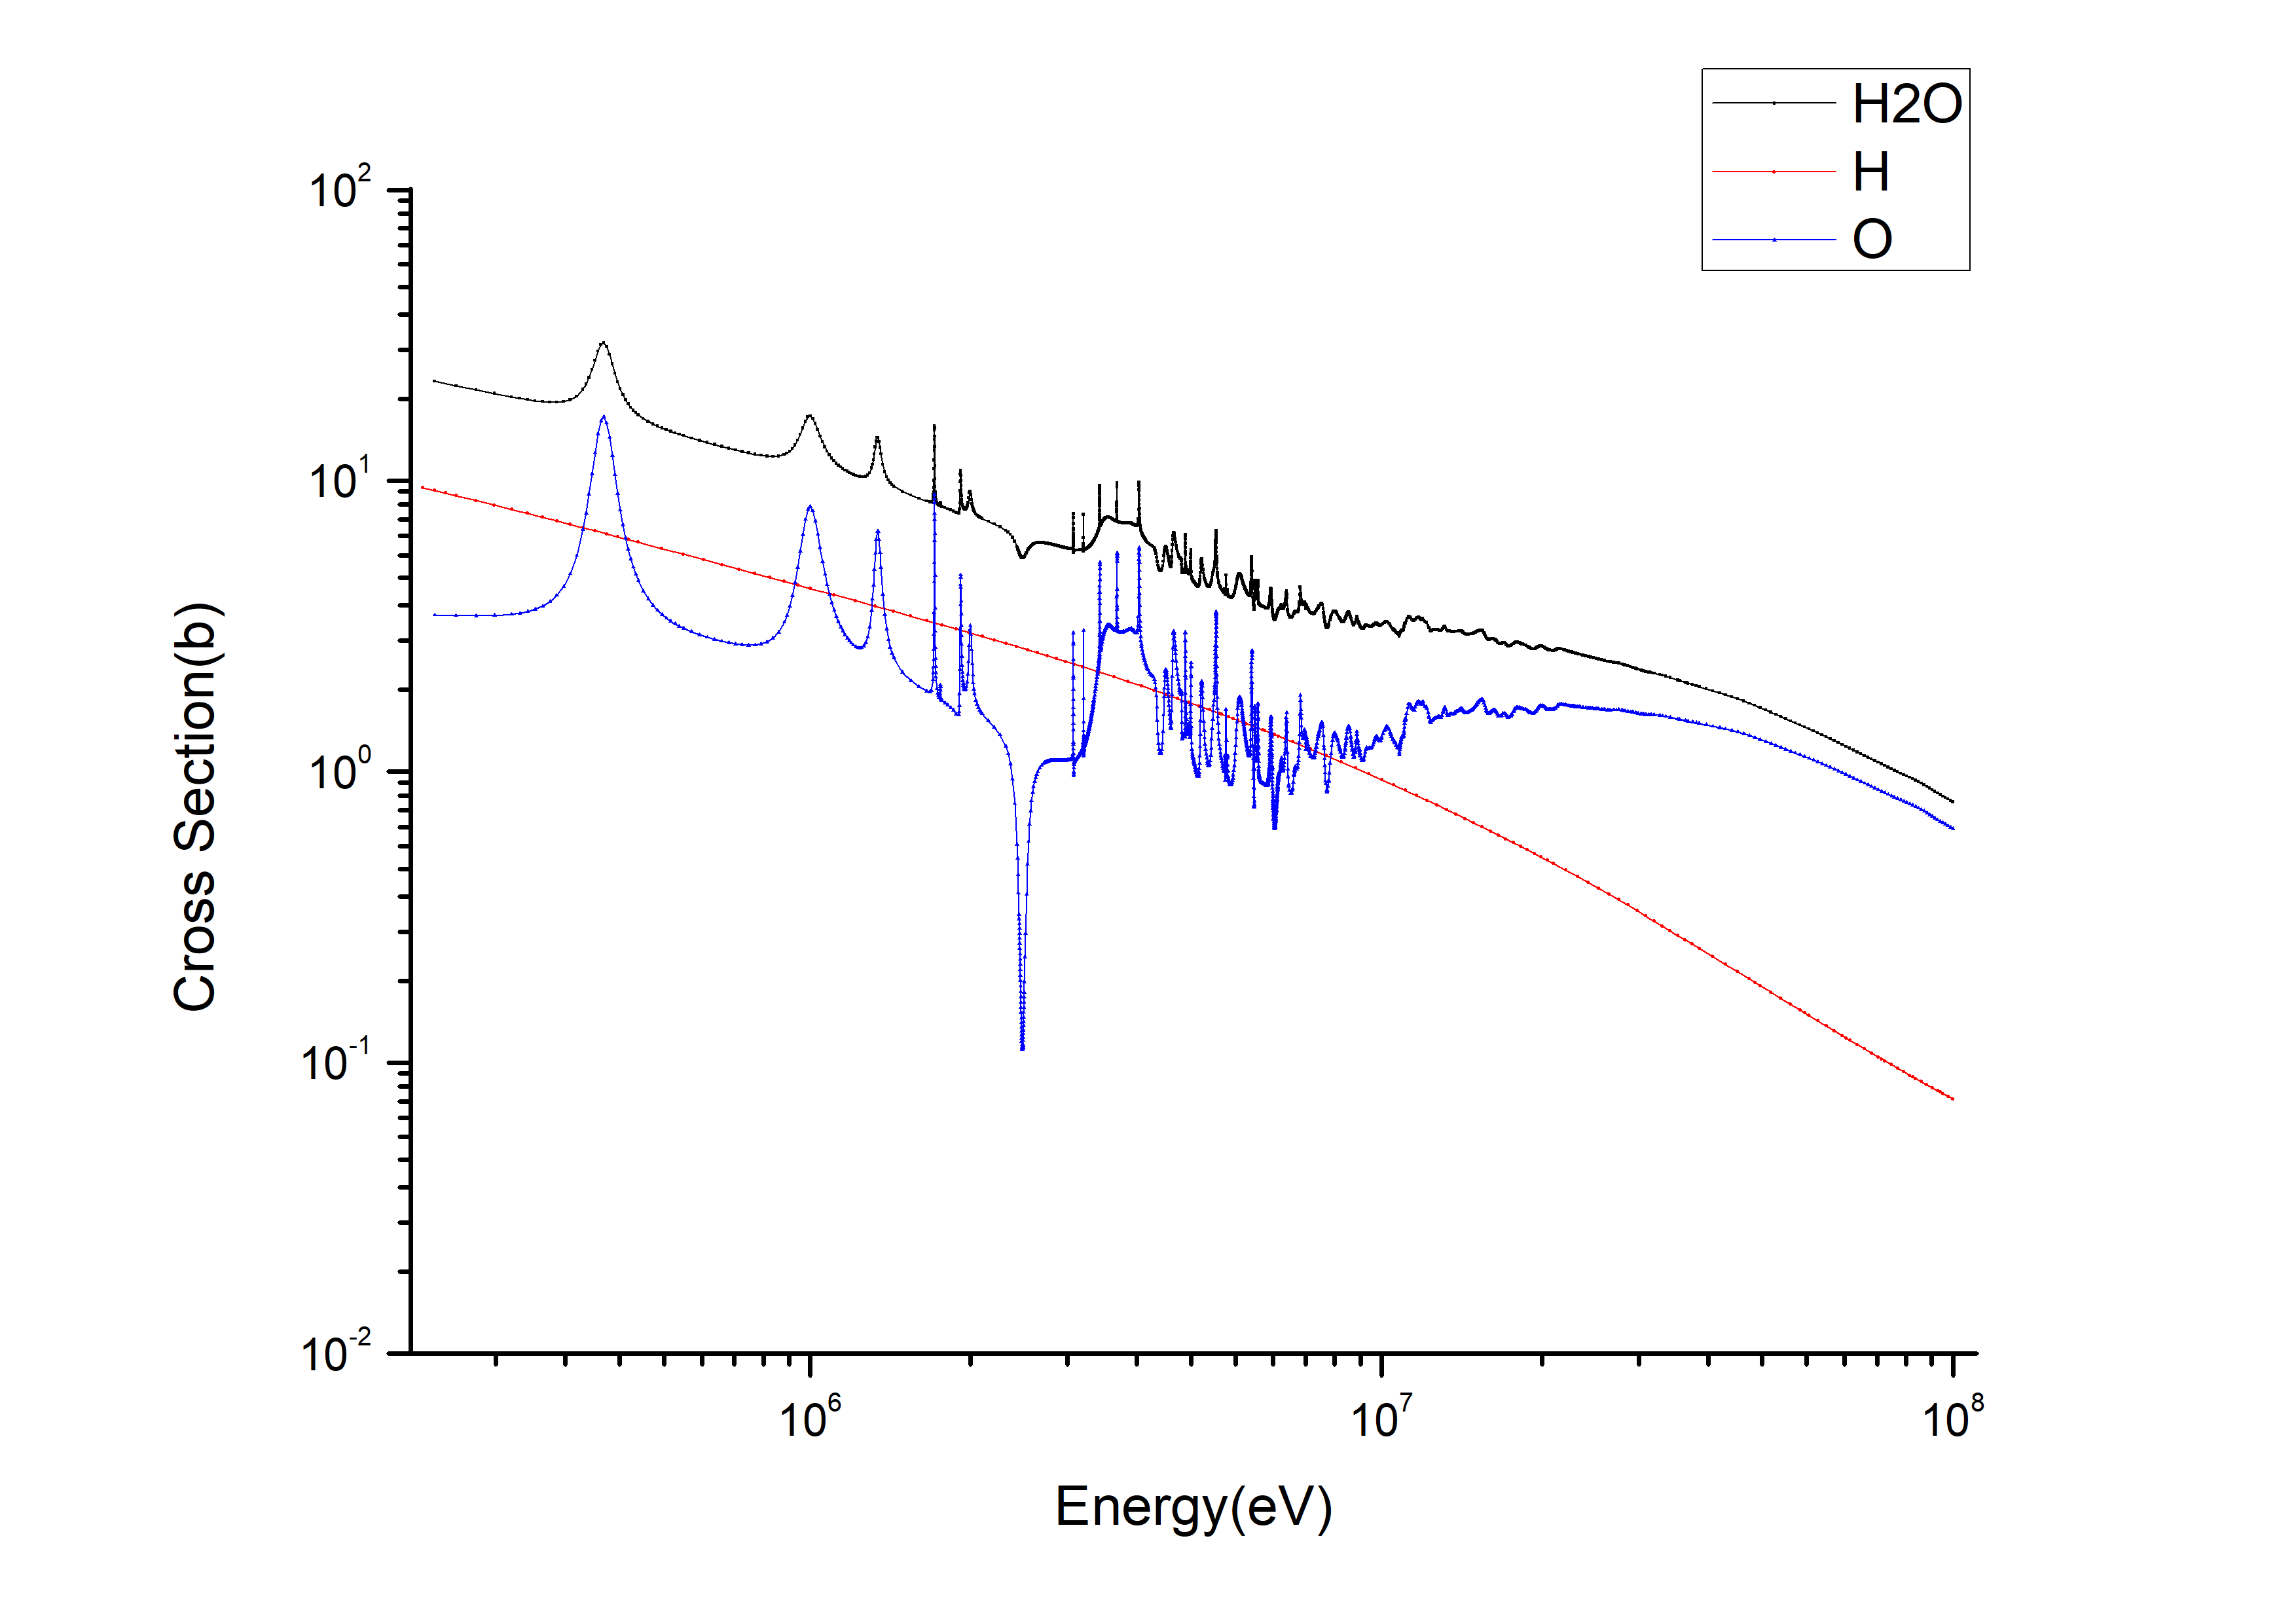
\includegraphics[width=\textwidth]{img/Neutron section in water interpolate based O.png}
    \caption{以$^{16}O$的能量点插值}
    \label{fig:water_o}
\end{figure}

\section{对公式$ \Psi = \begin{cases}
1 - e^{-\frac{x}{\mu}} & \quad \mu > 0 \\
1 - e^{-\frac{x-1}{\mu}} & \quad \mu < 0
\end{cases}$ 进行绘图,要求:\\
\textcircled{1} \quad 取固定的$\mu$值,绘出$\Psi$与$x$的关系图像;\\
\textcircled{2} \quad 取固定的$x$值,绘出$\Psi$与$\mu$的关系图像。}
\textcircled{1} $\mu$值分别取$[-1, -\frac{5}{7}, -\frac{3}{7}, -\frac{1}{7}, \frac{1}{7}, \frac{3}{7}, \frac{5}{7}, 1]$时,绘出$\Psi$与$x$的关系图像如图\ref{fig:Psi_x}所示:
\begin{figure}[H]
    \centering
    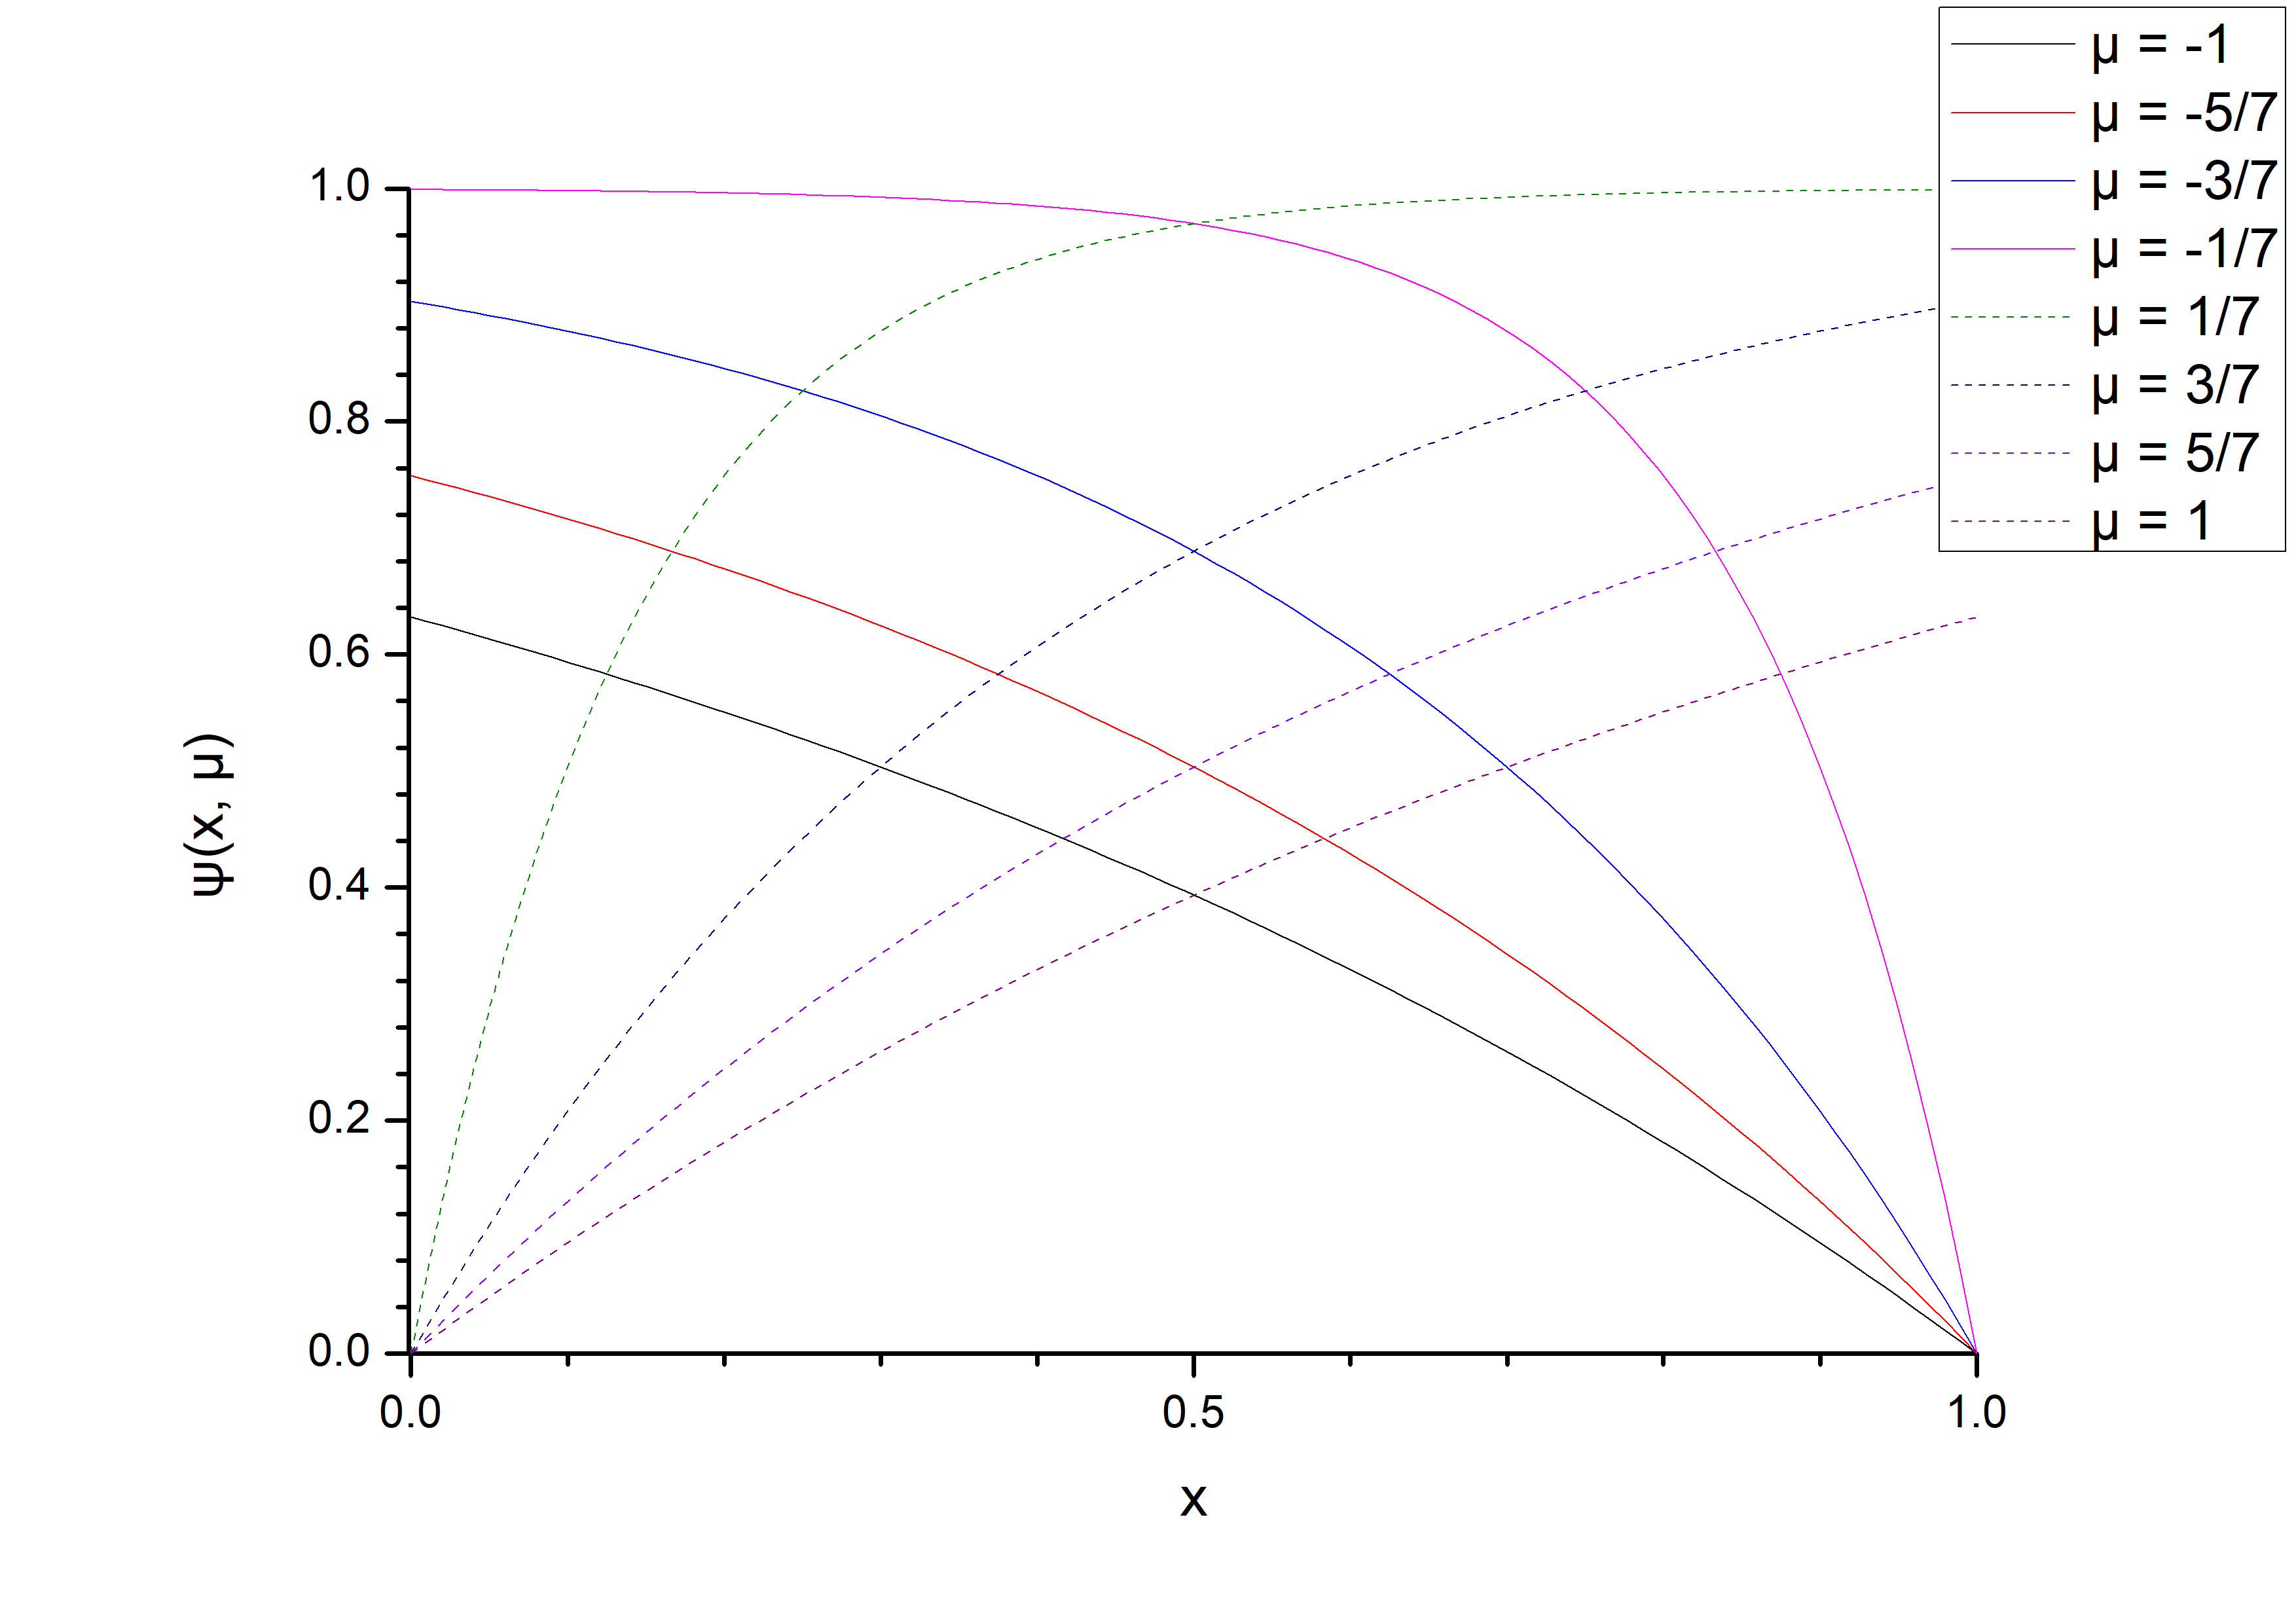
\includegraphics[width=\textwidth]{img/psi_x1.png}
    \caption{$\Psi$与$x$的关系图像}
    \label{fig:Psi_x}
\end{figure}
\textcircled{2} $x$值分别取$[0.1, 0.2, 0.3, 0.5, 0.7, 0.8, 1.0]$时,绘出$\Psi$与$\mu$的关系图像如图\ref{fig:Psi_mu}所示:
\begin{figure}[H]
    \centering
    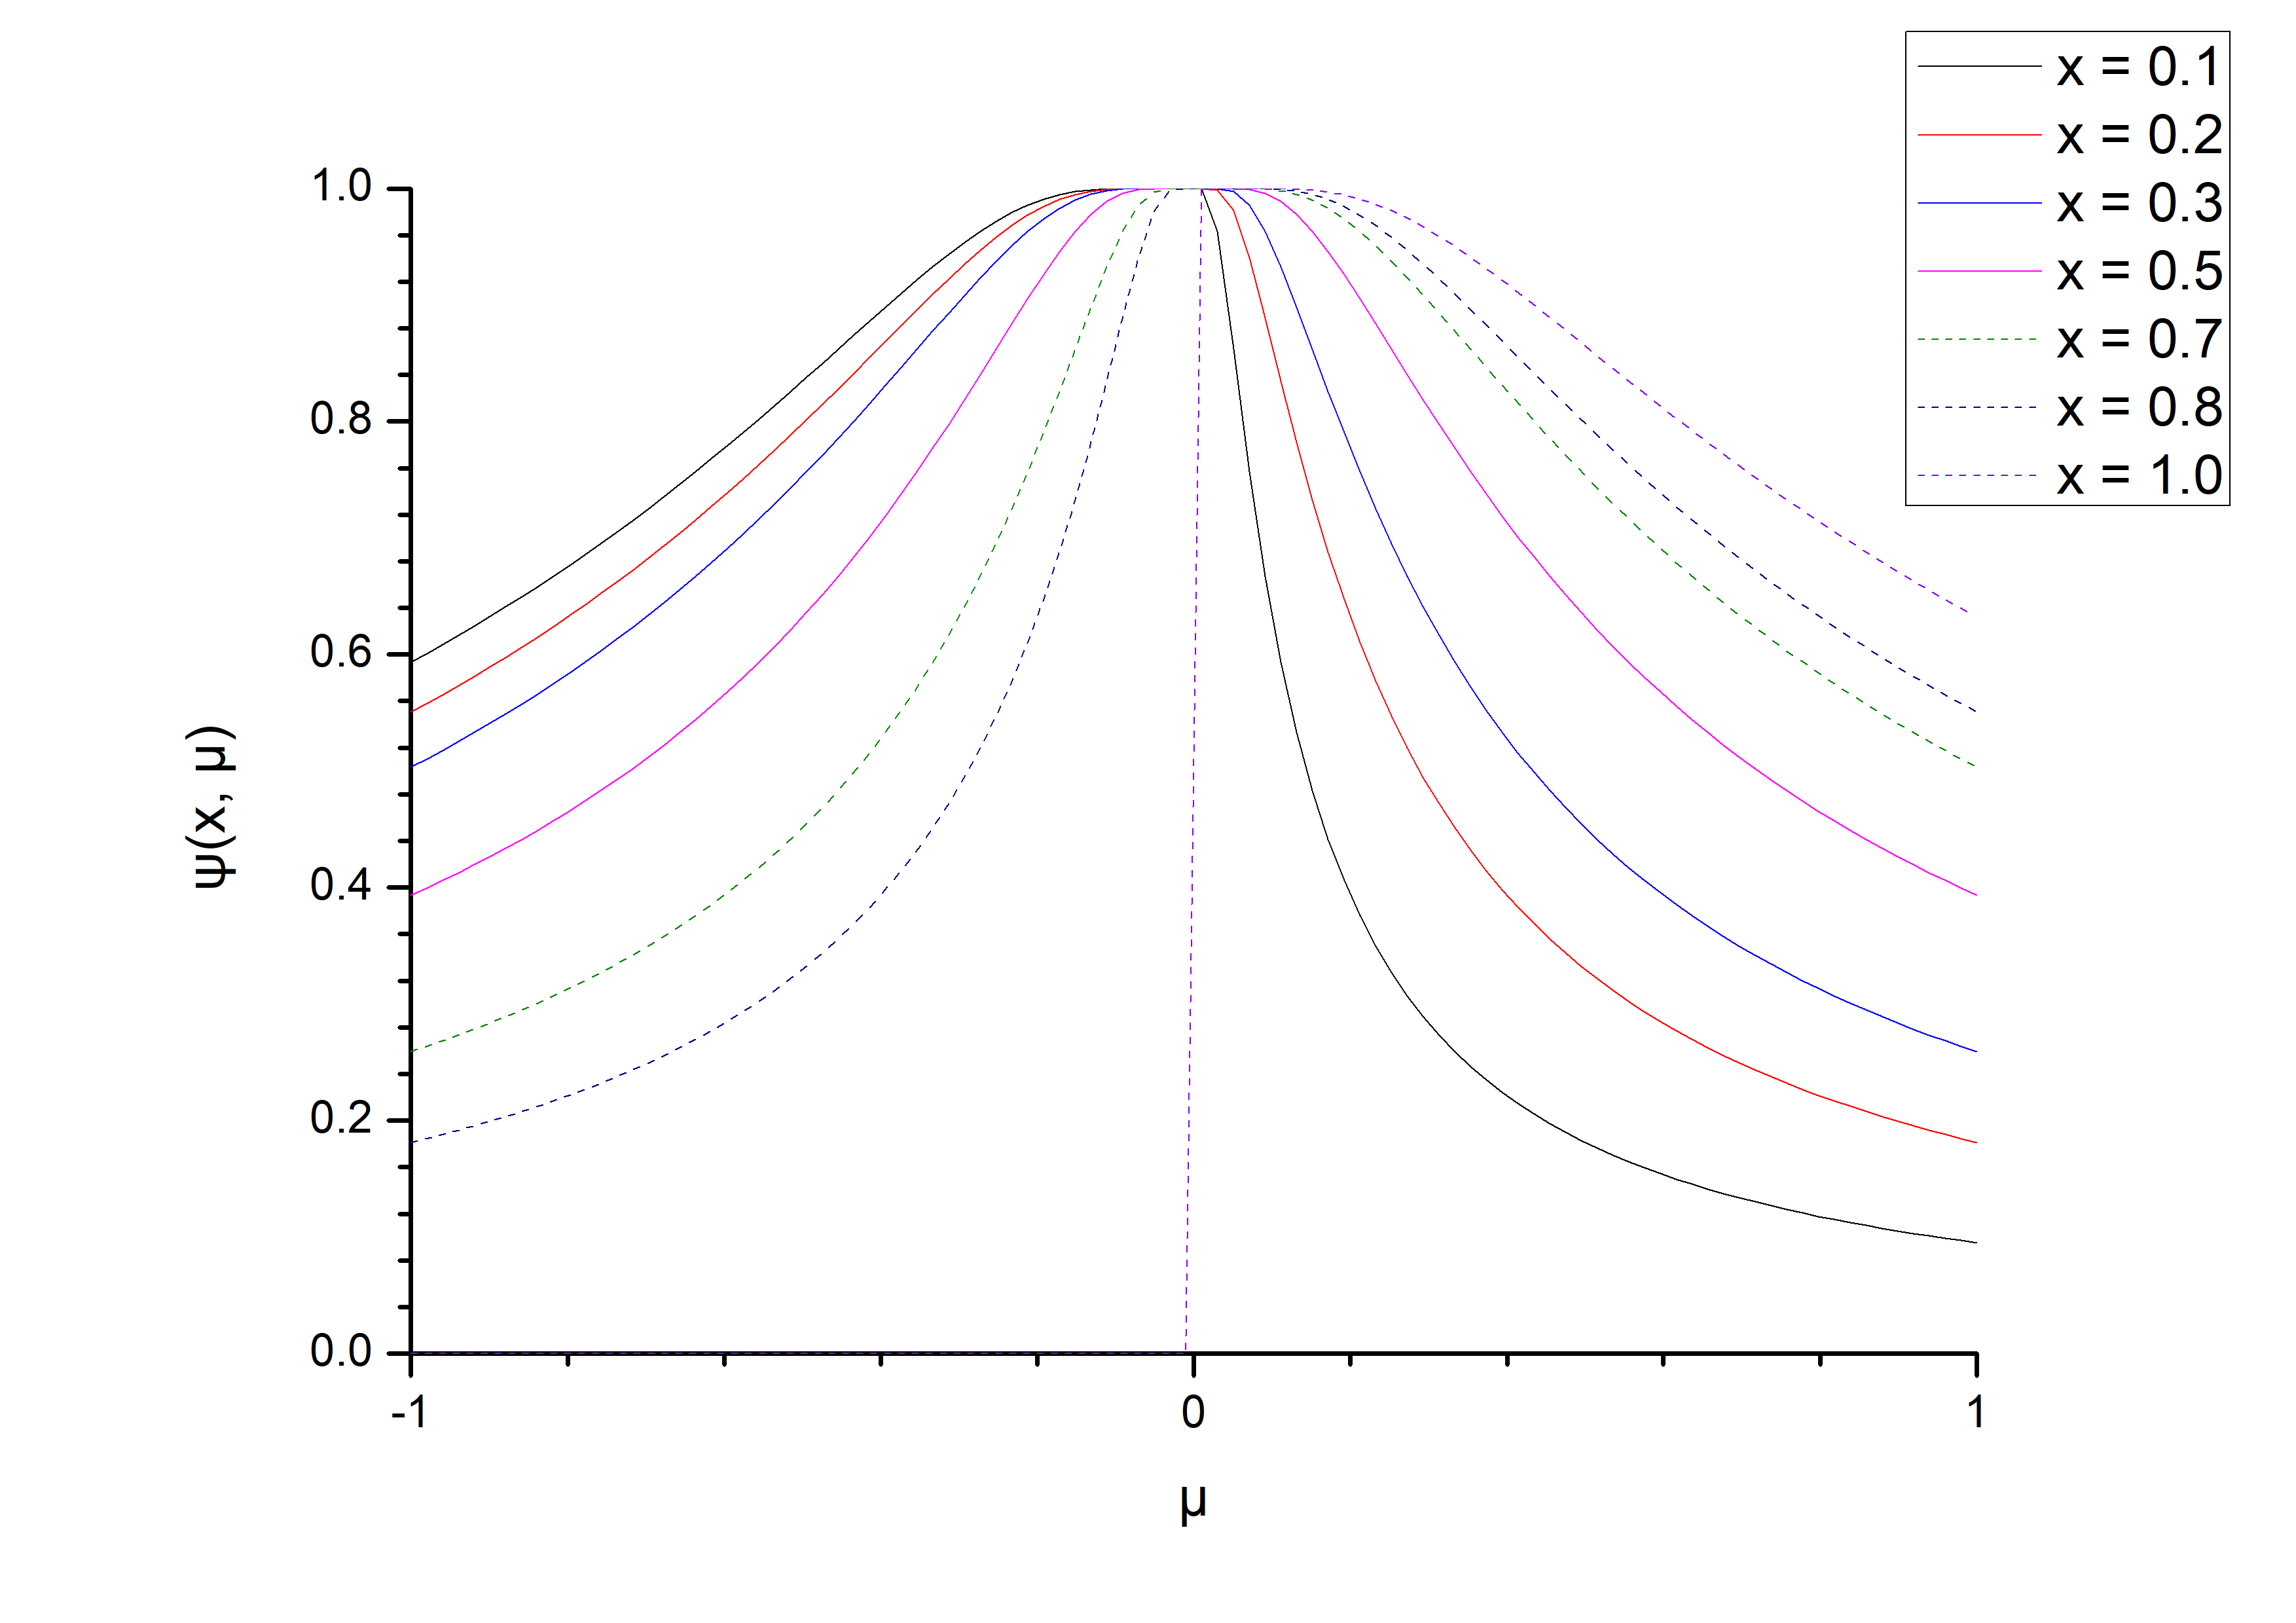
\includegraphics[width=\textwidth]{img/psi_mu1.png}
    \caption{$\Psi$与$\mu$的关系图像}
    \label{fig:Psi_mu}
\end{figure}

\section{\textcircled{1} \quad 查询$\Gamma$函数相关资料, \\
\textcircled{2} \quad 对公式 $\Psi = 
\begin{cases}
1 - e^{-\frac{x}{\mu}} & \quad \mu > 0 \\
1 - e^{-\frac{x-1}{\mu}} & \quad \mu < 0
\end{cases}$进行$\mu \in (-1, 1)$的积分$\Phi(x) = 2\pi \int_{-1}^{1} \Psi(x, \mu)\, \mathrm{d}\mu$,积分结果$\Phi(x)$用$\Gamma$函数表示出来,并绘出$\Phi(x)$与$x \in (0, 1)$的关系图像。}
\textcircled{1} $\Gamma$函数可以通过欧拉(Euler)第二类积分定义:
$$\Gamma(z) = \int_0^\infty t^{z-1}e^{-t}\,\mathrm{d}t$$
对于复数$z$,我们要求$Re(z) > 0$ \\
在数学中,上不完全$\Gamma$函数和下不完全$\Gamma$函数,是$\Gamma$函数的推广。它们的定义分别如下:
$\Gamma(s,x) = \int_x^\infty t^{s-1}e^{-t} \, \mathrm{d}t.$ \qquad
$\gamma(s,x) = \int_0^x t^{s-1}e^{-t} \, \mathrm{d}t.$ \qquad
$\Re(s) > 0, x \in \mathbb{R}_0^+$ \\
且有递推关系:$\Gamma(s, x) = (s - 1)\Gamma(s-1, x) + x^{s-1}e^{-x}$
\par
\textcircled{2} \begin{align*}
    \Phi(x) & = 2\pi \int_{-1}^{1} \Psi(x, \mu)\, \mathrm{d}\mu \\  
    & = 2 \pi \int_{-1}^{0}\Psi(x, \mu)\, \mathrm{d}\mu + 2 \pi \int_{0}^{1} \Psi(x, \mu)\, \mathrm{d}\mu \\
    & = 2 \pi \int_{-1}^0 1 - e^{-\frac{x-1}{\mu}} \, \mathrm{d}\mu + 2 \pi \int_0^1 1 - e^{-\frac{x}{\mu}} \, \mathrm{d}\mu \\
\end{align*}
令$t = \frac{x - 1}{\mu}$,则
\begin{align*}
    2 \pi \int_{-1}^0 1 - e^{-\frac{x-1}{\mu}} \, \mathrm{d}\mu 
    & = 2 \pi [1 - (1-x) \int_{1-x}^\infty t^{-2}e^{-t}\,\mathrm{d}t] \\
    & = 2 \pi [1 - (1-x) \Gamma(-1, 1-x)] \\
    & = 2 \pi [1 + (1-x) \Gamma(0, 1-x) - e^{x-1}]
\end{align*}
同理,令$t = \frac{x}{\mu}$,则
\begin{align*}
    2 \pi \int_{0}^1 1 - e^{-\frac{x}{\mu}} \, \mathrm{d}\mu
    & = 2 \pi [1 - x \int_{x}^\infty t^{-2}e^{-t}\,\mathrm{d}t] \\
    & = 2 \pi [1 - x \Gamma(-1, x)] \\
    & = 2 \pi [1 + x \Gamma(0, x) - e^{-x}]
\end{align*}
故$\Phi(x) = 2 \pi [2 - e^{x-1} - e^{-x} + (1-x) \Gamma(0, 1-x) + x \Gamma(0, x)]$,绘出$\Phi$与$x \in (0, 1)$的关系图像如图\ref{fig:Phi_x}所示:
\begin{figure}[H]
    \centering
    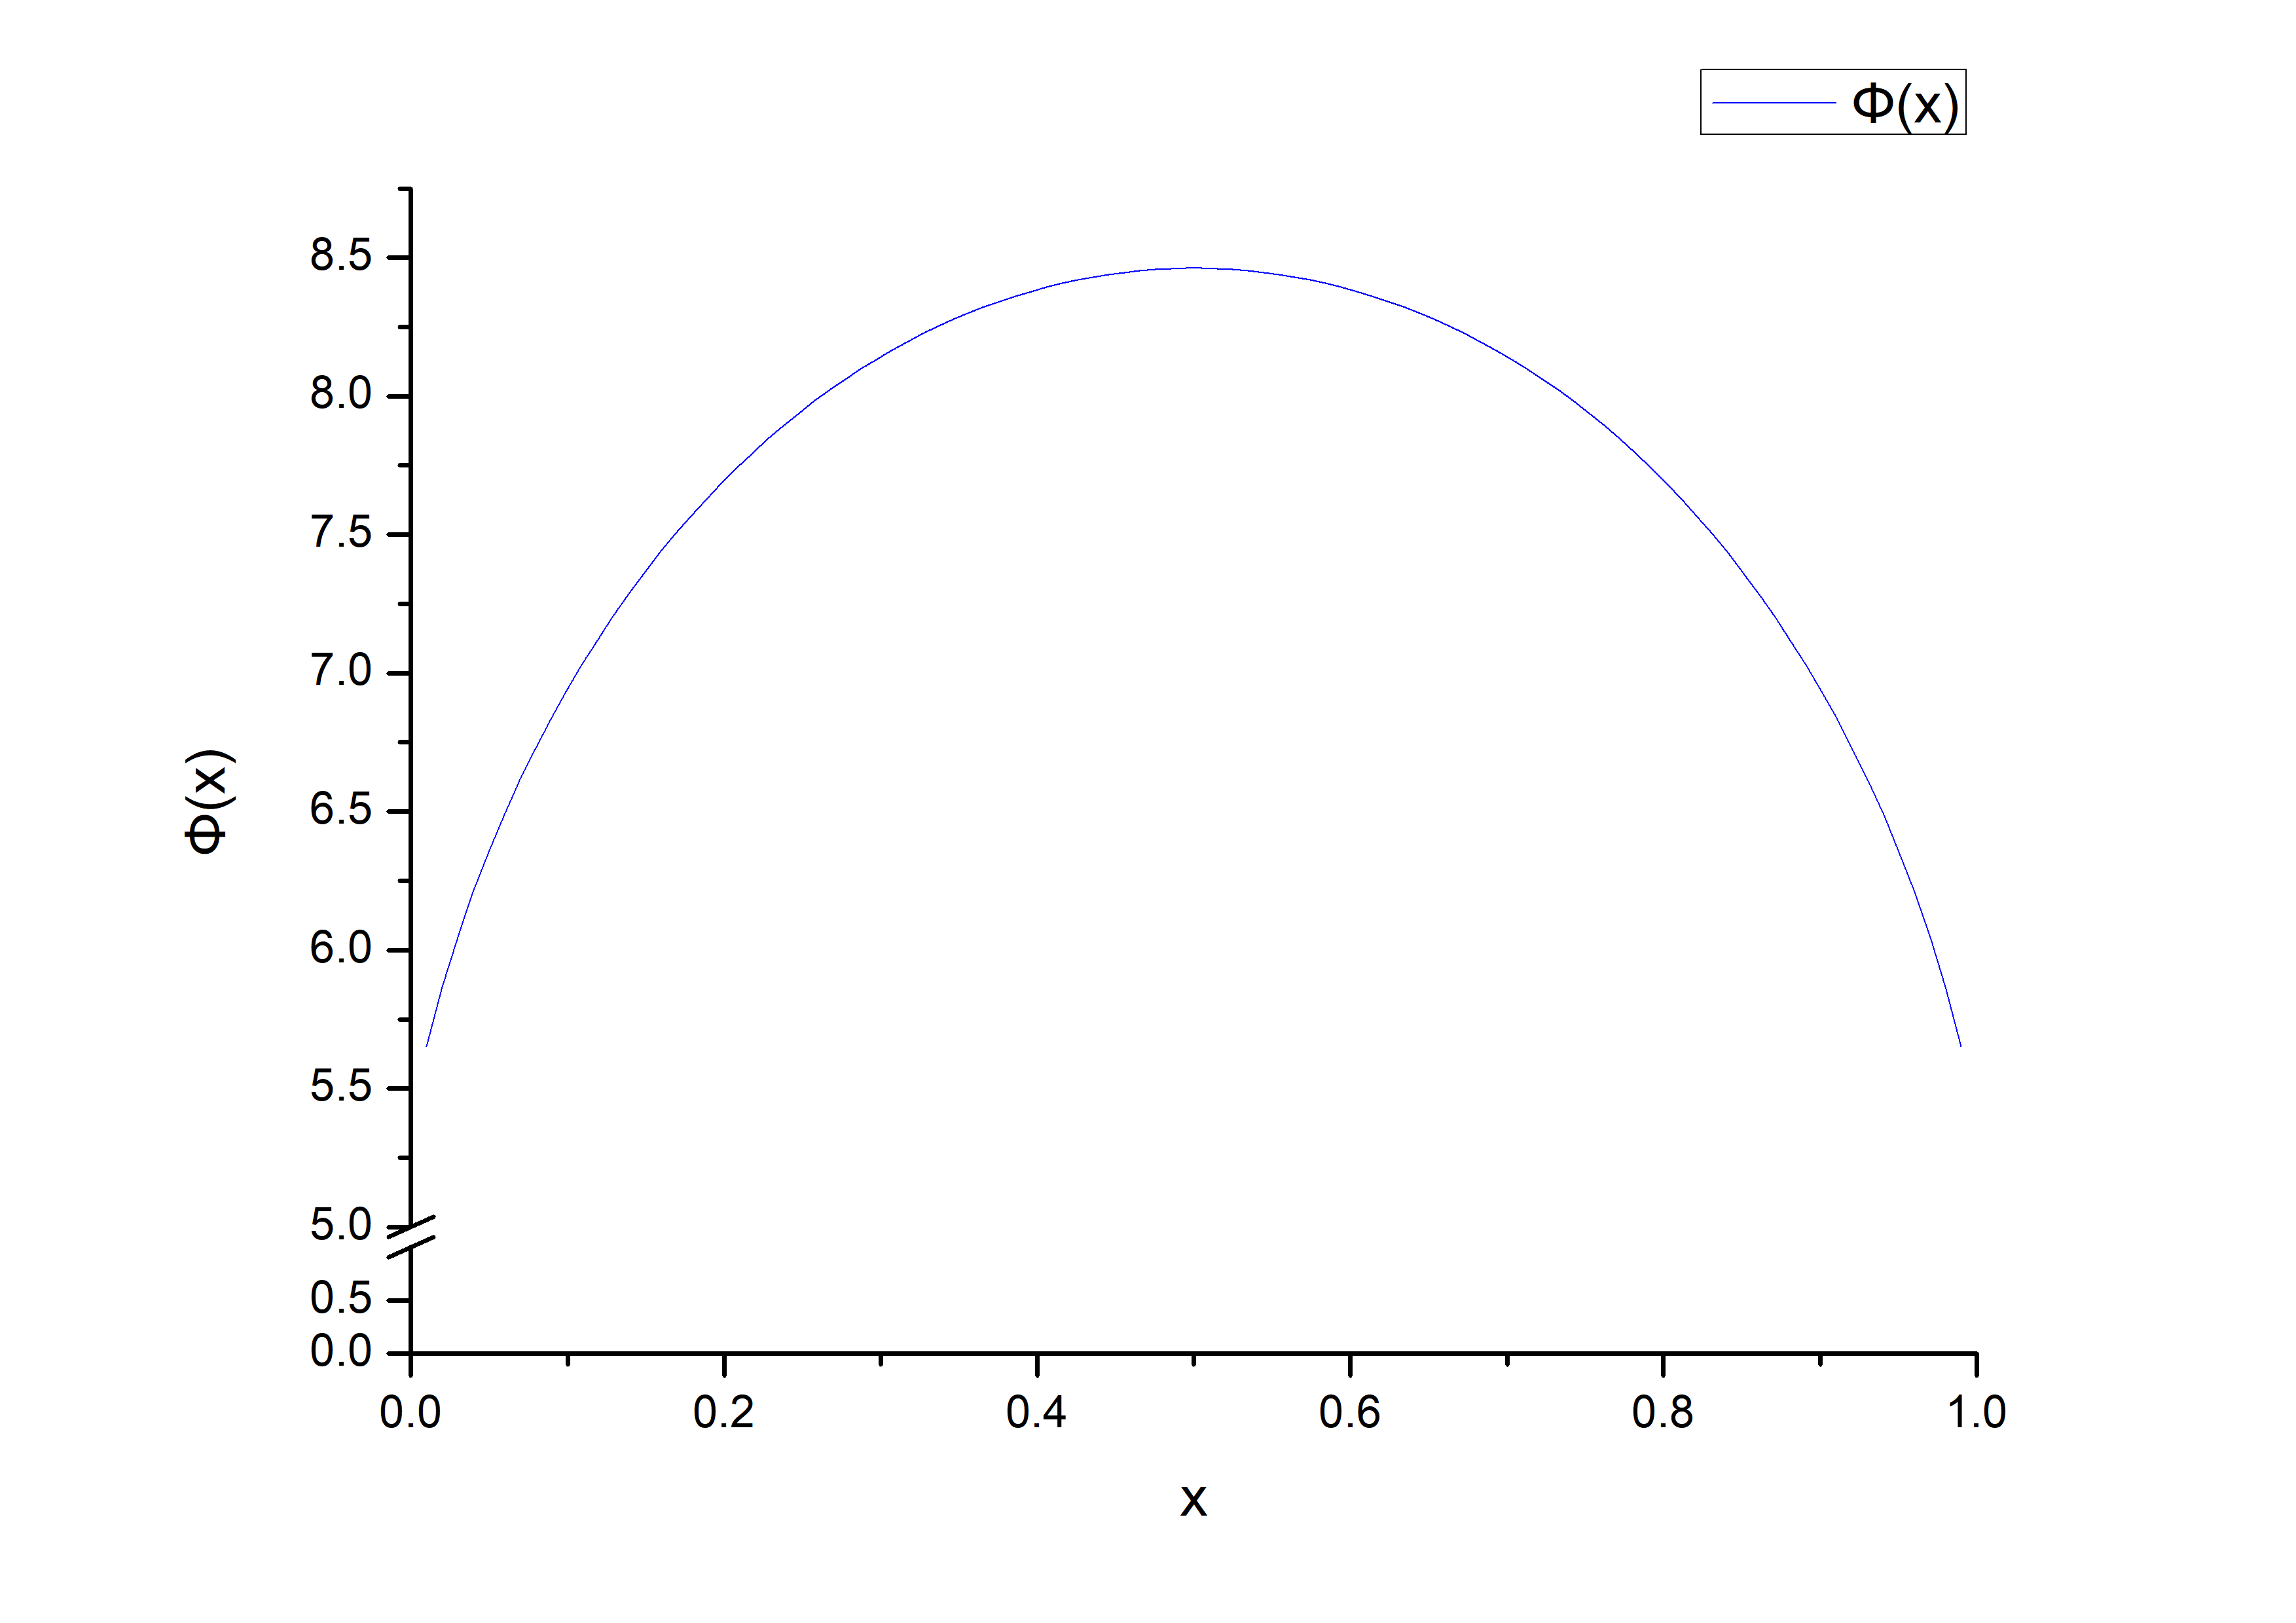
\includegraphics[width=\textwidth]{img/phi_x1.png}
    \caption{$\Phi$与$x$的关系图像}
    \label{fig:Phi_x}
\end{figure}

\end{document}